% !TeX spellcheck = en_US
\thispagestyle{empty}
\begin{tikzpicture}[remember picture, overlay, inner sep=10pt]
  \iftoggle{noartbackground}{}{
    \node(cover)[anchor=center] at (current page.center) {
      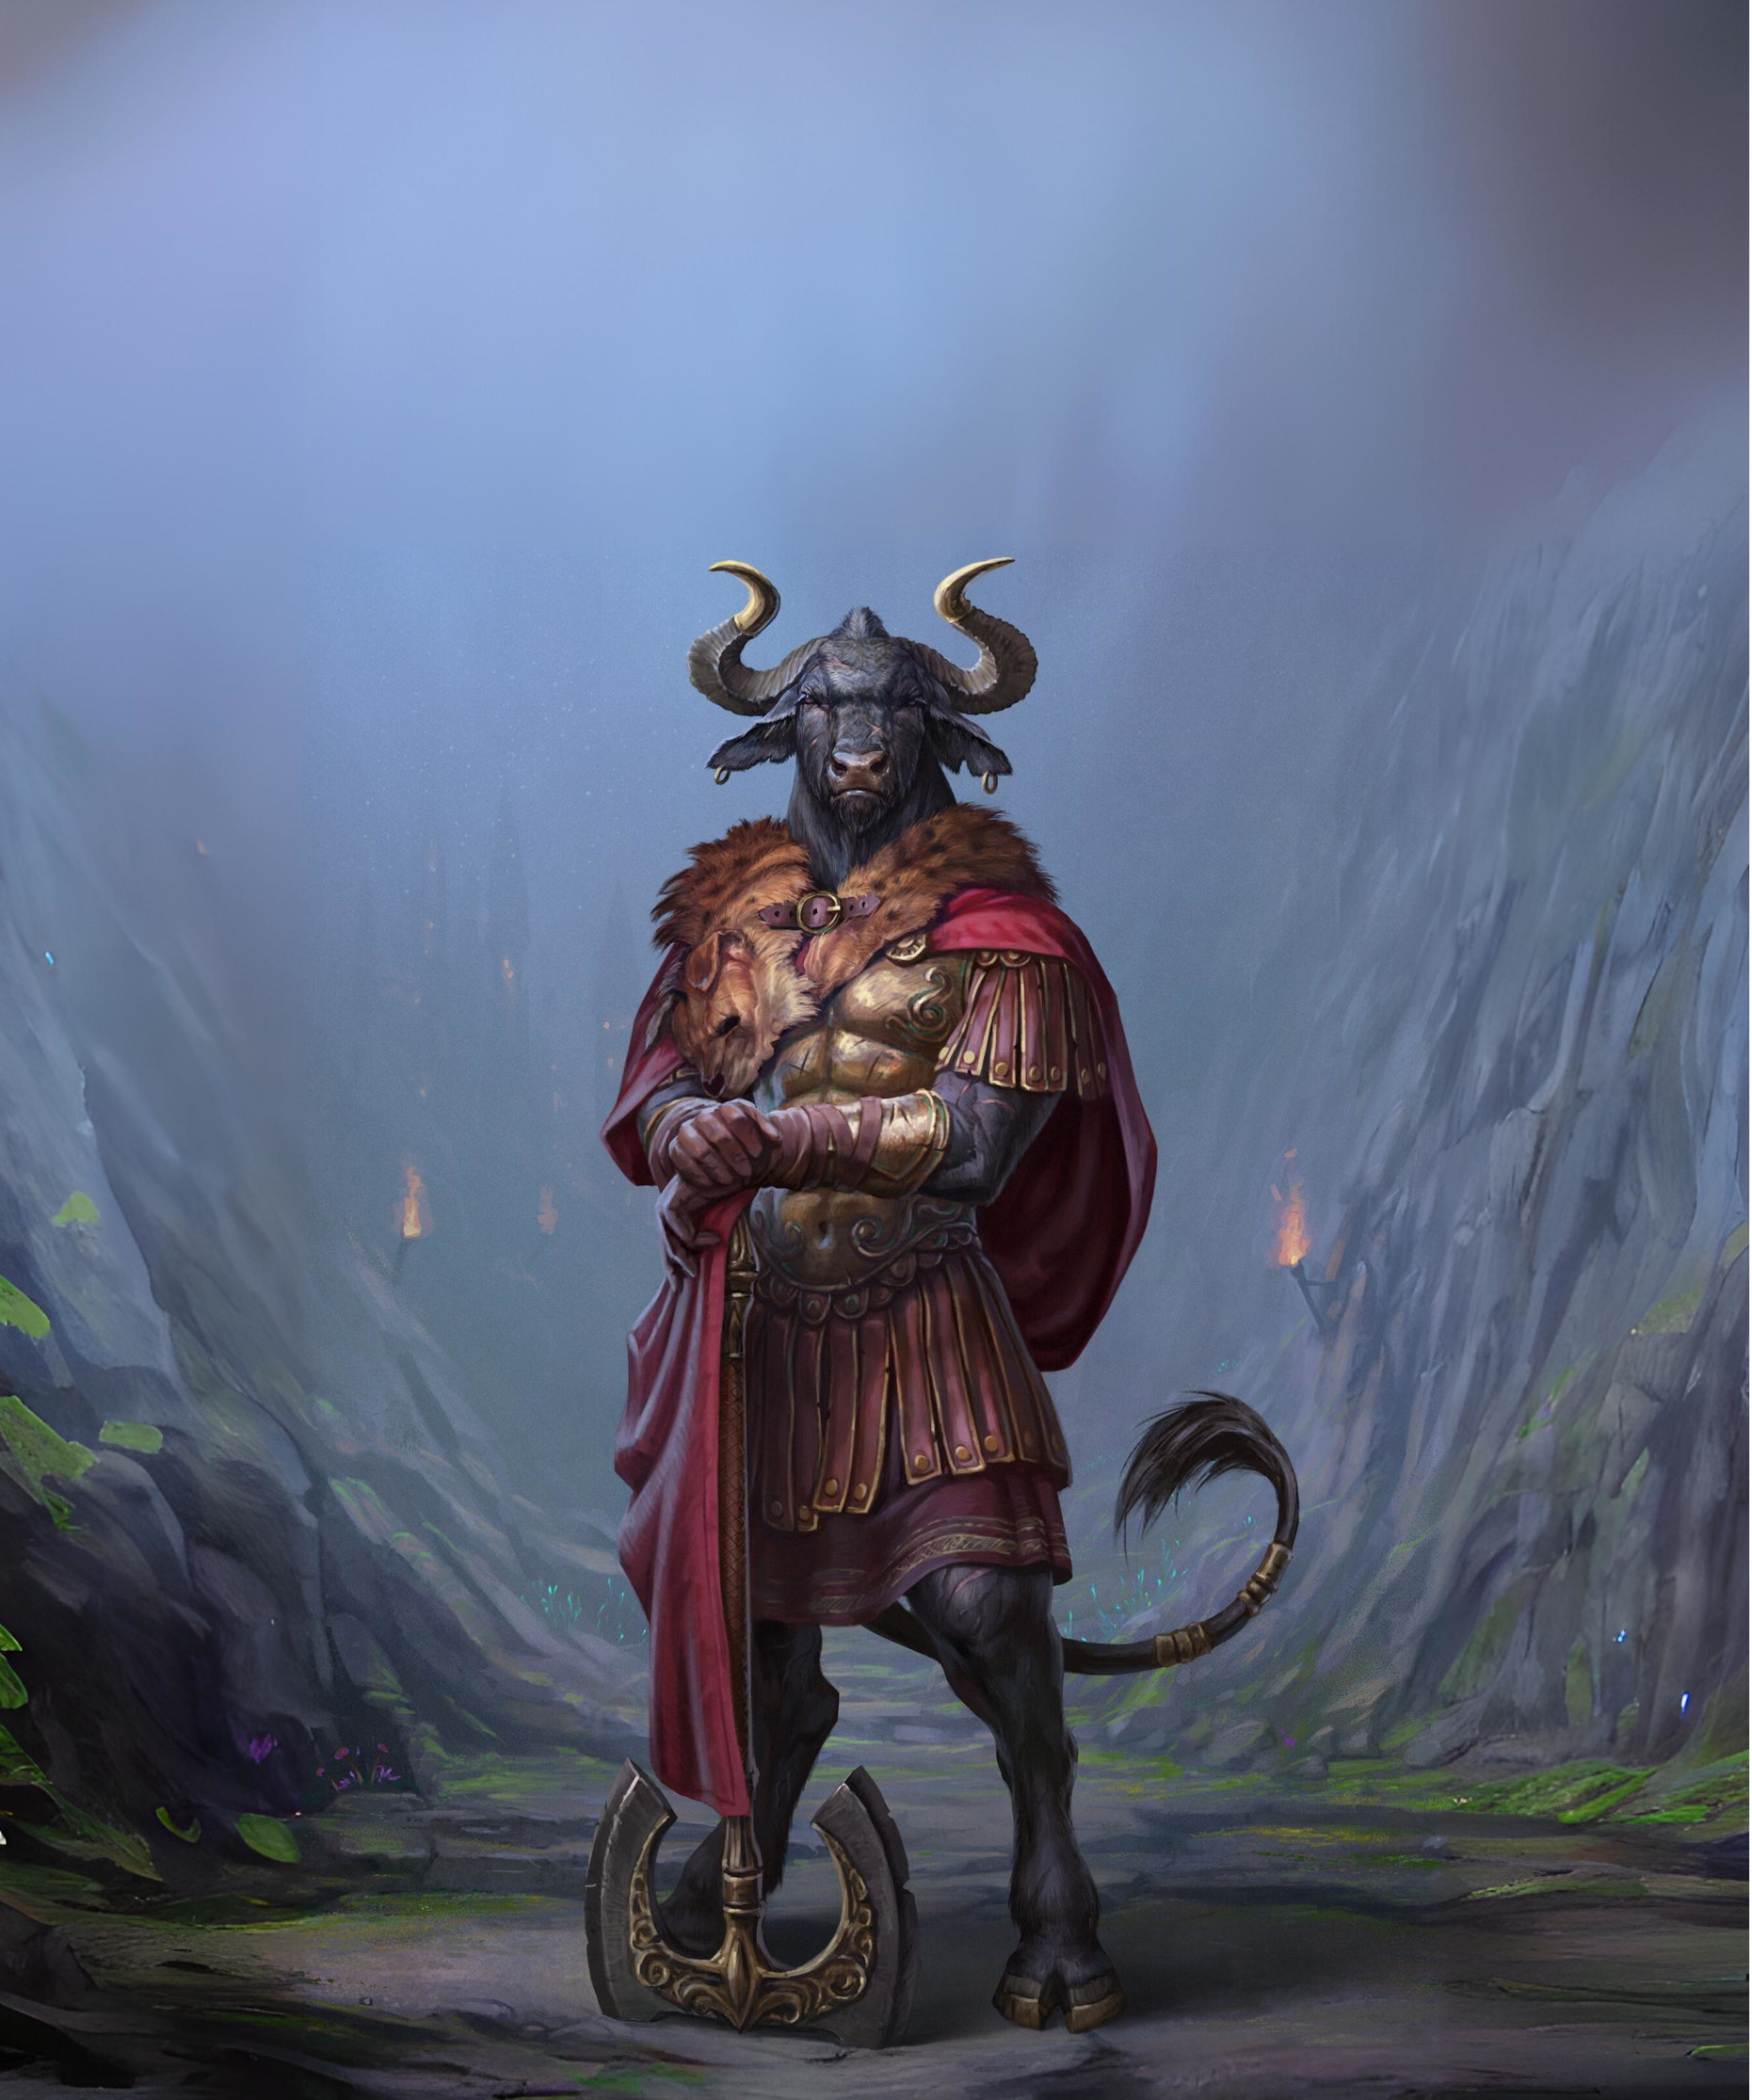
\includegraphics[height=\paperheight, keepaspectratio]{\layout/cover.jpg}
    };
  }
  \node(title)[minimum width = \paperwidth, anchor=center, yshift=\dimexpr-10em\relax] at (current page.north) {
    
\includegraphics[width=0.6\paperwidth]{\layout/cover_title.png}
  };
  \node(subtitle)[anchor=center, yshift=12em] at (current page.south) {
    
\includegraphics[width=0.6\paperwidth]{\layout/cover_subtitle.png}
  };
\end{tikzpicture}

% Render phantom SVGs before their use in tabular env
\phantom{
  \includesvg[height=0.1px]{\svgs/bronze.svg}
  \includesvg[height=0.1px]{\svgs/bronze.svg}
  \includesvg[height=0.1px]{\svgs/silver.svg}
  \includesvg[height=0.1px]{\svgs/golden.svg}
  \includesvg[height=0.1px]{\svgs/azure.svg}
  \includesvg[height=0.1px]{\svgs/gold.svg}
  \includesvg[height=0.1px]{\svgs/building_materials.svg}
  \includesvg[height=0.1px]{\svgs/valuables.svg}
  \includesvg[height=0.1px]{\svgs/attack_yellow.svg}
  \includesvg[height=0.1px]{\svgs/defense_yellow.svg}
  \includesvg[height=0.1px]{\svgs/damage-table.svg}
}
